%FOR PDFLATEX USE ONLY
\documentclass[a4paper,12pt]{article}

\usepackage{amssymb,amsmath} %math symbols

\usepackage[margin=2cm]{geometry} %paper geometry

\usepackage[utf8]{inputenc} %allows unicode (including russian) source file
\usepackage[russian]{babel} %docment in russian-style
\usepackage[utf8]{inputenc}
%\usepackage[unicode]{hyperref} %links inside of the text
\usepackage[pdftex]{graphicx} %includegraphics pictures
\usepackage{cmlgc} %bold text

\usepackage{array} %arrays

%\usepackage{wrapfig}
%\usepackage{array}
%\usepackage{lipsum}
%\usepackage{esvect}
%\usepackage{hyperref}

\usepackage{subfig}
%\usepackage{calc}
%\usepackage{pgfplots,tikz,circuitikz}
%\usepackage{tkz-euclide}
\usepackage{booktabs}
\usepackage{multirow}

\usepackage{wrapfig}

\begin{document}

\begin{center}
  \LARGE{Работа 4.3.1}\\[0.2cm]
  \LARGE{Изучение дифракции света}\\[0.2cm]
  \large{Малиновский Владимир}\\[0.2cm]
  \normalsize{\texttt{galqiwi@galqiwi.ru}}
\end{center}

\textbf{Цель работы}: исследовать являения дифракции Френеля и Фраунгофера на щели, изучить влияние дифракции на разрешающую способность оптических инструментов.


\textbf{В работе используются}: оптическая скамья, ртутная лампа, монохроматор, щели с регулируемой шириной, рамка с вертикальной нитью, двойная щель, микроскоп на поперечных салазках с микрометрическим винтом, зрительная труба.
\section*{Описание работы}
\subsection*{А. Дифракция Френеля}
\begin{figure}[h]
\includegraphics[scale=0.7]{0.png}
\centering
\caption{Схема установки 1.}
\end{figure}
Схема установки представлена на Рис. 1. Световые лучи освещают щель $S_2$ и испытывают на ней дифракцию. Дифракционная картина рассматривается с помощью микроскопа М, сфокусированного на некоторую плоскость наблюдения П. Щель $S_2$ освещается параллельным пучком монохроматического света с помощью коллиматора, образованного объективом $O_1$ и щелью $S_1$, находящейся в его фокусе. На $S_1$ сфокусированно изображение спектральной линии, выделенной из спектра ртутной лампы Л при помощи монохроматор $C$, в котором используется призма прямого зрения. \\
Распределение интенсивности света в плоскости П рассчитаем с помощью зон Френеля. При освещении $S_2$ параллельным пучком лучей (плоская зона) зоны Френеля представляют собой плоскости, параллельные краям щели. Результирующая амплитуда в точке наблюдения определеяется суперпозицией колебаний от тех зон Френеля, которые не перекрыты створками щели. Графическое определение результирующей амплитуды производится с помощью векторной диаграммы -- спирали Корню. Суммарная ширина $m$ зон Френеля $z_m$ определяется соотношение
\begin{equation}
z_m = \sqrt{am\lambda},
\end{equation}
где $a$ -- расстояние от щели до плоскости П. Вид наблюдаемой картины определяется \textit{числом Френеля} $\Phi$:
$$
\Phi^2 = \dfrac{D}{\sqrt{a\lambda}}
$$
-- число зон Френеля, которые укладываются в ширине щели $D$. $p = \frac{1}{\Phi^2}$ называется \textit{волновым параметром}. Дифракционной картины нет, когда П совпадает с плоскостью щели. При малом удалении от щели $\Phi \gg 1$ и картина наблюдается в узкой убласти на границе света и тени у краёв экрана. При последующих удалениях две группы дифракционных полос перемещаются независимо и каждая образует картину дифракции Френеля на экране. Распределение интенсивности может быть найдено с помощью спирали Корню. При дальнейшем увеличении $a$ две системы полос сближаются и накладываются друг на друга, распределение интенсивности определяется числом зон Френеля в полуширине щели. Если их $m$, то будет набюдаться $m-1$ тёмная полоса.
\subsection*{Б. Дифракция Фраунгофера на щели}
\begin{wrapfigure}{r}{0.5\textwidth}
  \begin{center}
    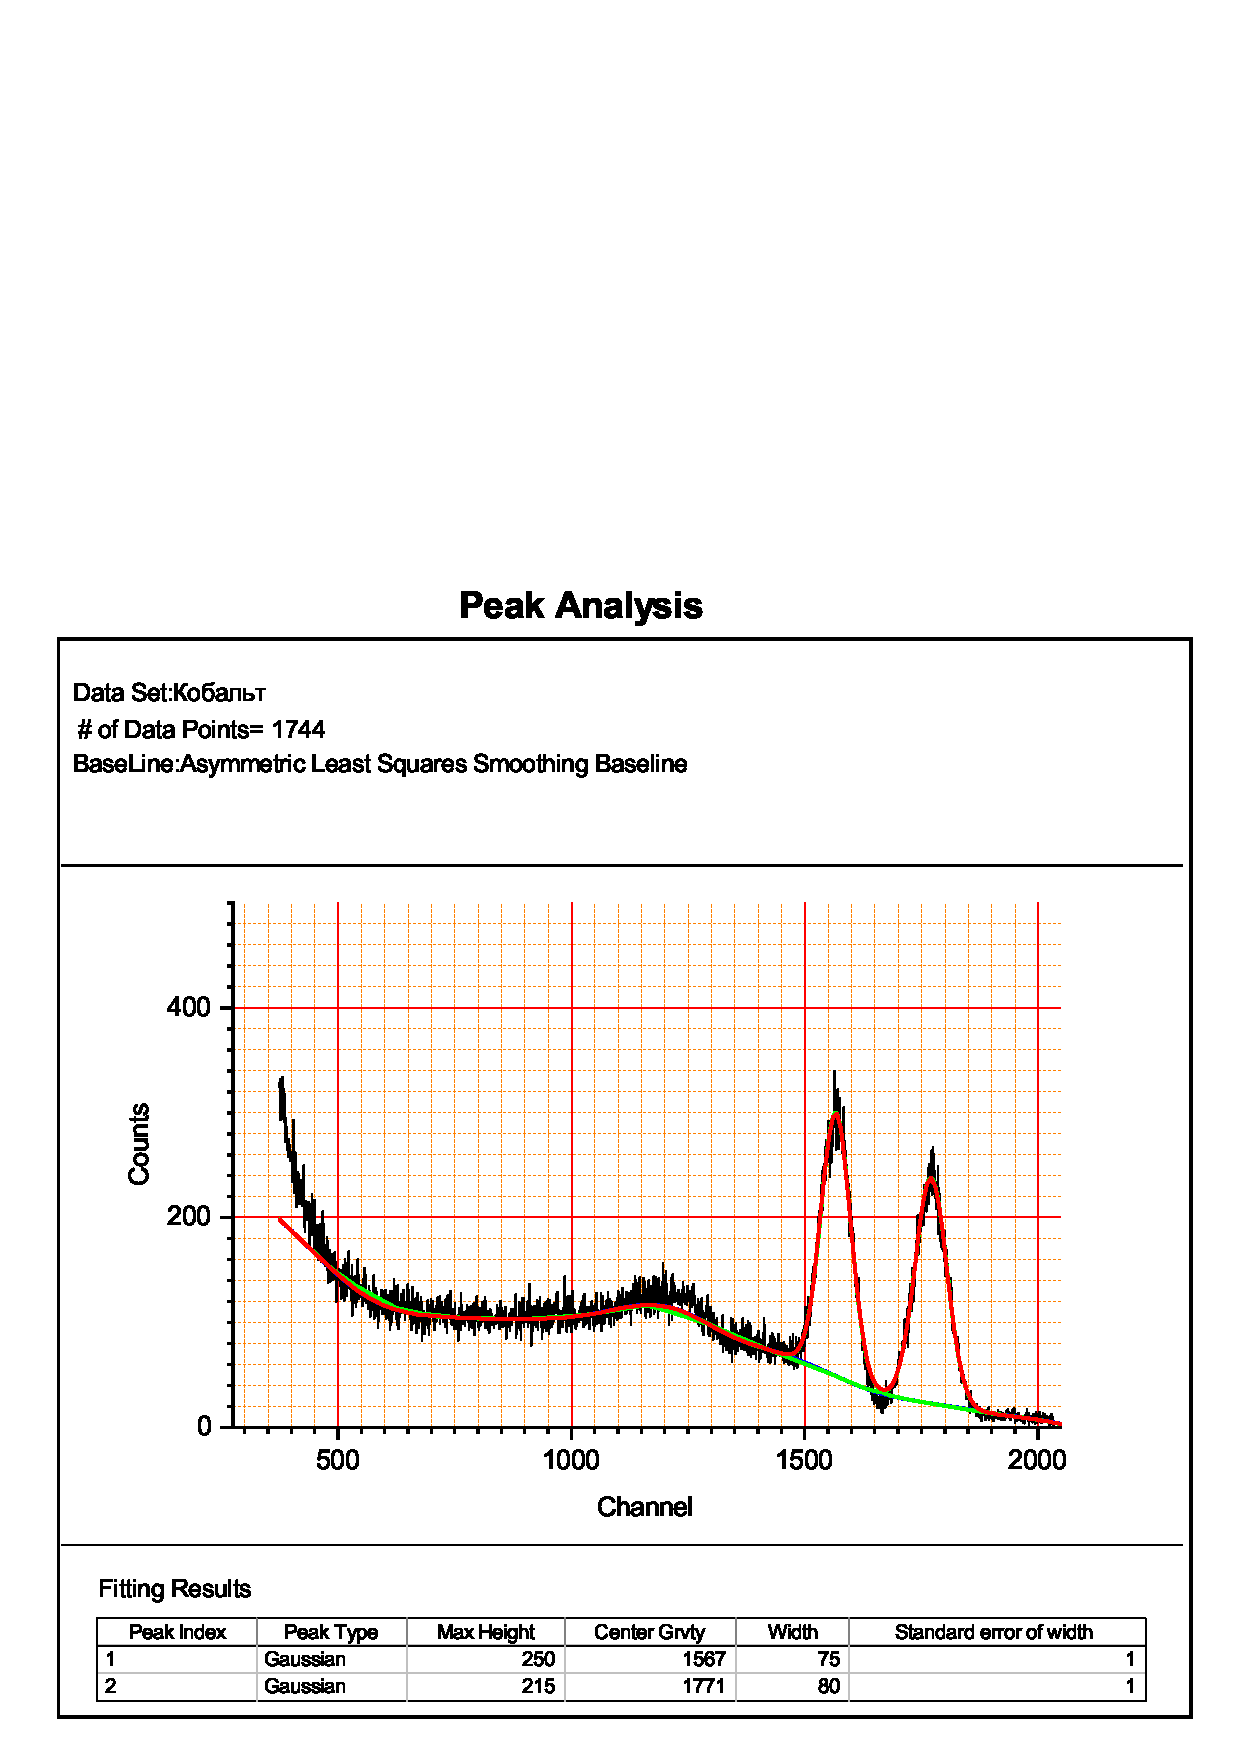
\includegraphics[width = 0.4\textwidth]{2.png}
  \end{center}
  \caption{Построение зон Френеля}
\end{wrapfigure}
Для выкладок ниже нам потребуется знать \textit{принцип Гюйгенса-Френеля}. Он формулируется следующим образом:\\
\textit{Каждый элемент волнового фронта можно рассматривать как центр  вторичного возмущения, порождающего вторичные сферические волны, а результирующее световое поле  в каждой точке пространства будет определяться интерференцией этих волн.}\\
Теперь рассмотрим первое применение этого принципа, получившее название \textit{метод зон Френеля}

\begin{wrapfigure}{r}{0.3\textwidth}
  \begin{center}
    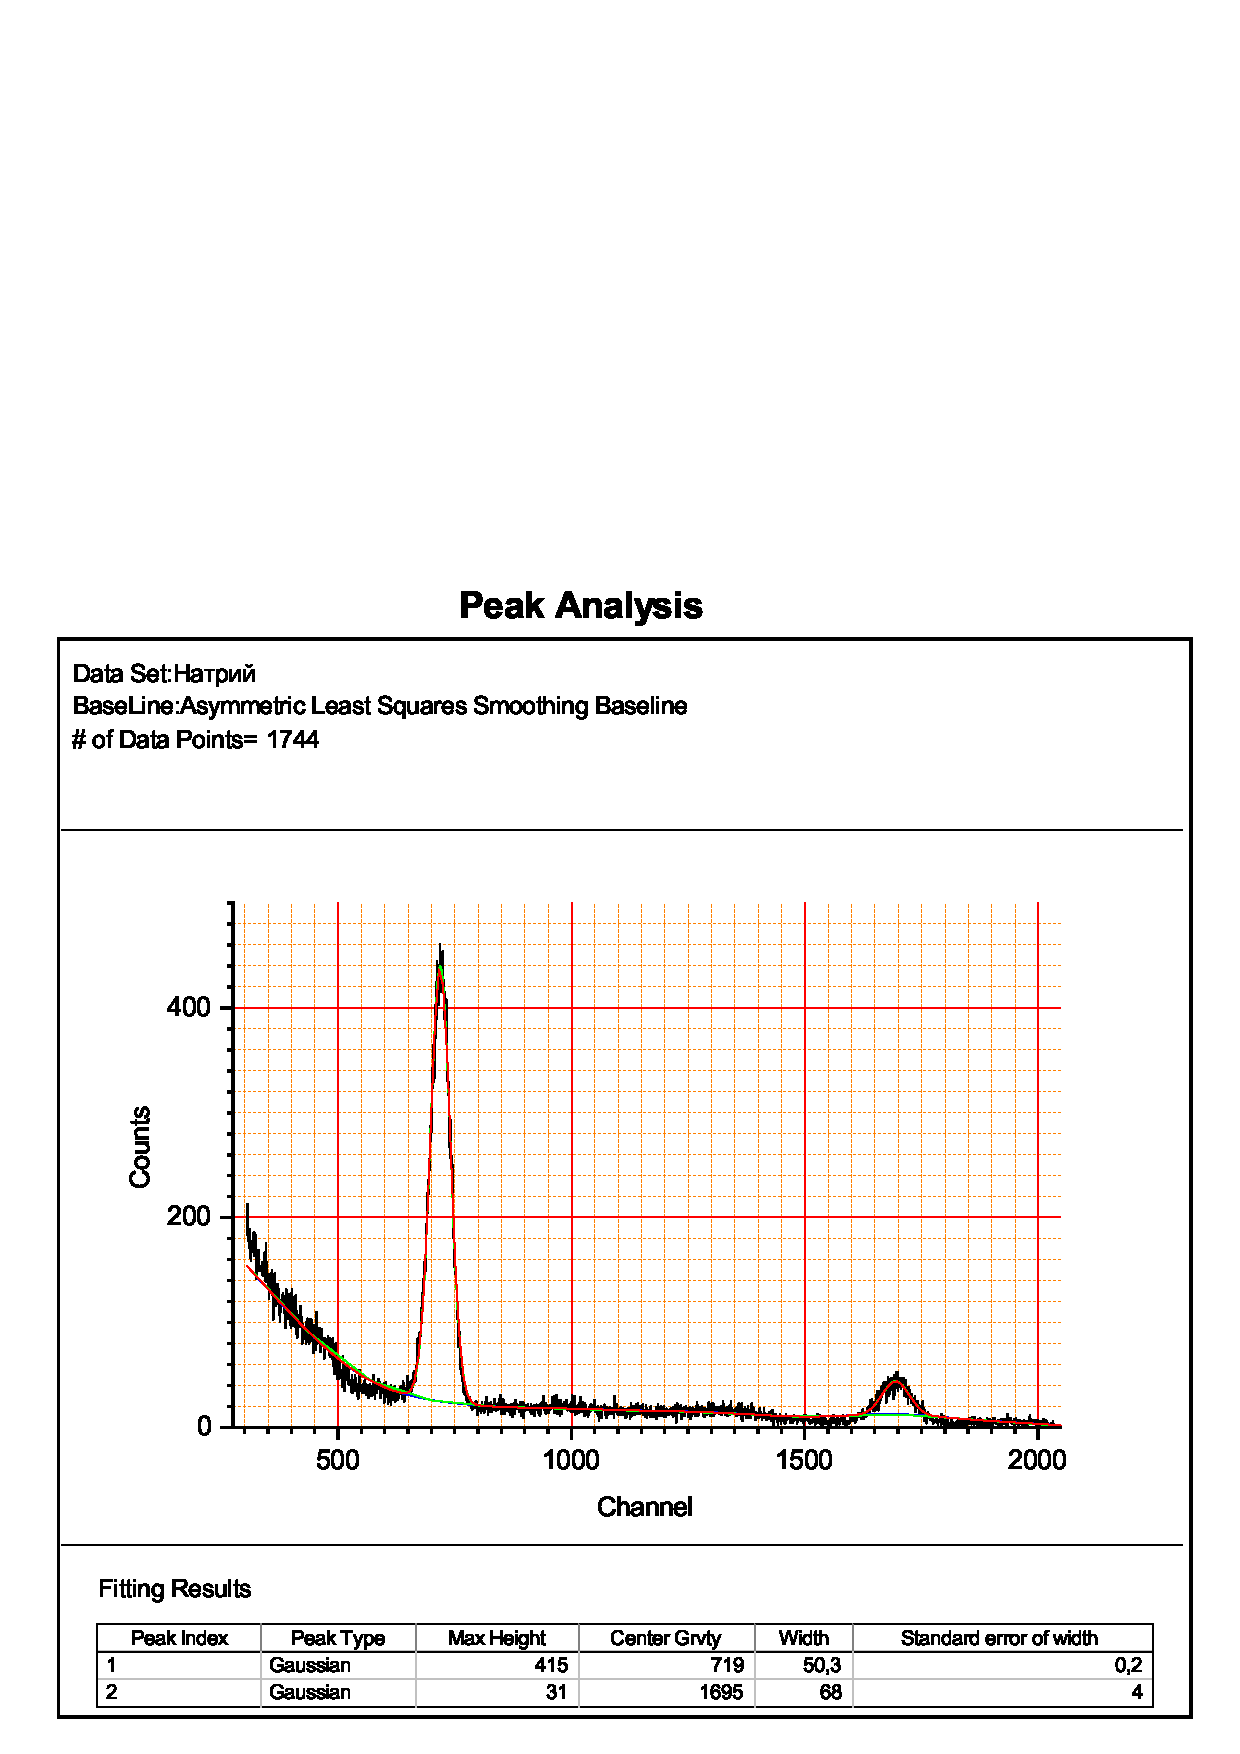
\includegraphics[width = 0.3\textwidth]{1.png}
  \end{center}
  \caption{К фазовым соотношениям при дифракции Фраунгофера}
  \vspace{+30pt}
\end{wrapfigure}

Для этого рассмотрим действие световой волны действующей из точки $A$ в какой-то точке $B$.
В этом случае можно, взяв точку $M_0$ в качестве центра (см. рис. 1), построить ряд концентрических сфер, радиусы которых начинаются с $b$ и увеличиваются каждый раз на половину длины волны $\frac{\lambda}{2}$. При пересечении с плоским фронтом волны $F$ эти сферы дадут концентрические окружности. Таким образом, на фронте волны появятся кольцевые зоны (зоны Френеля) с радиусами $r_1, r_2$ и т. д.

Из геометрических соображений посчитав, можно получить, что 
\begin{equation}
r_i = i \sqrt{a \lambda}
\end{equation}

Картина дифракции упрощается, когда ширина щели становится значительно меньше ширины первой зоны Френеля, т.е. если 
\begin{equation}
D \ll\sqrt{a \lambda} 
\end{equation}	
Это условие всегда выполняется при достаточно большом $a$. В этом случае говорят, что \textit{дифракция Фраунгофера}. Дифракционную картину в этом случае называются \textit{дифракцией Фраунгофера}. При выполнении пункта $(2)$ у нас упрощаются фазовые соотношения, что поясняет рис. 2, в итоге с хорошим приближением можно считать, что разность хода между крайними лучами, приходящими от щели в точке наблюдения $P$, с хорошим приближением равна 
\begin{equation}
\Delta = r_2 - r_1 \approx D \sin \theta \approx D \cdot \theta
\end{equation}
Здесь предполагается, что $\theta$ достаточно мал.
Дифракцию Фраунгофера можно наблюдать на установке Рис. 1, но для удобства к подобной установке добавляется объектив $O_2$.

\begin{figure}[h]
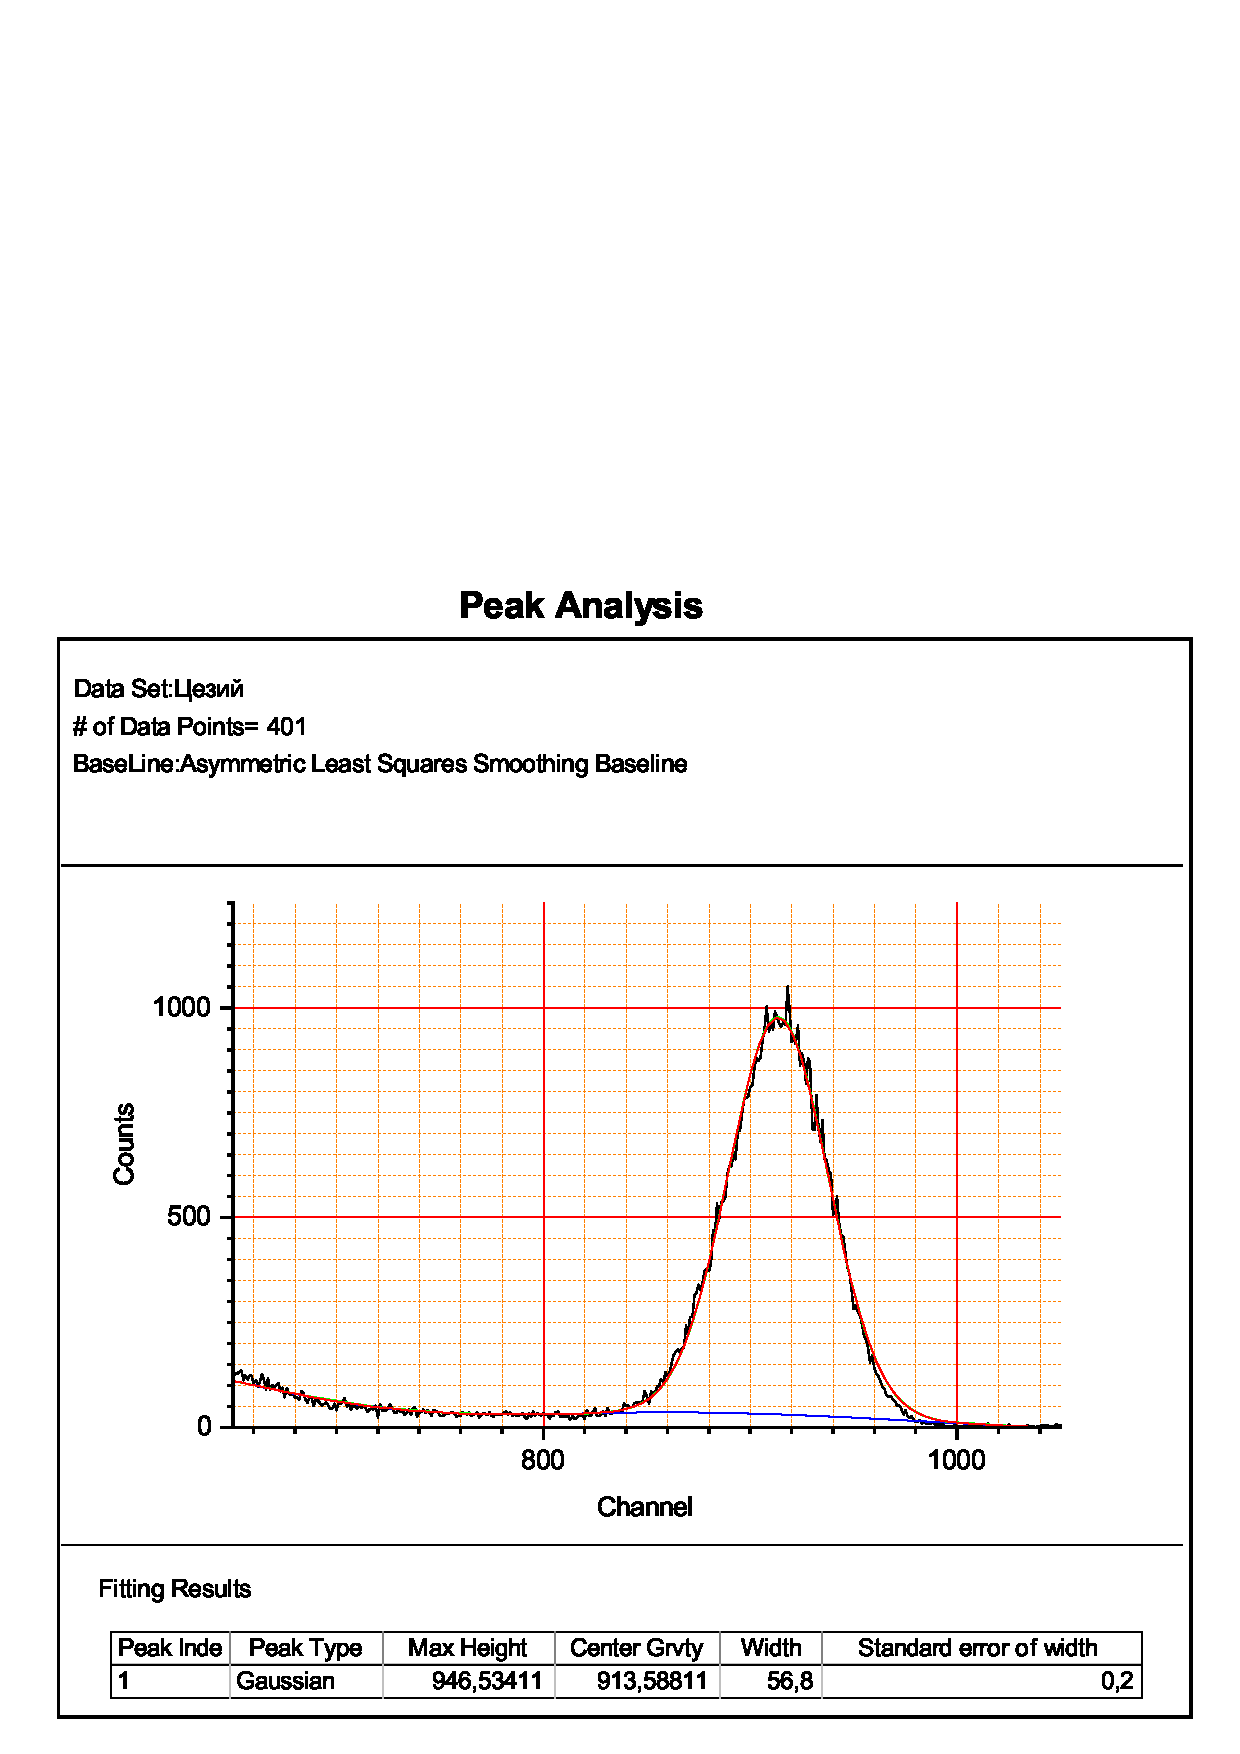
\includegraphics[width = 0.7\textwidth]{3.png}
\centering
\caption{Схема установки 2.}
\end{figure}
Дифракционная картина здесь наблюдается в фокальной плоскости объектива $O_2$. Каждому значению $\theta$ соответствует в этой плоскости точка, отстоящая от оптической оси на расстоянии 
\begin{equation}
X = f_2 \tan \theta \approx f_2 \theta.
\end{equation}
Объектив не вносит разности хода между интерферирующими лучам, поэтому в его фокальной плоскости наблюдается неискажённая дифракционная картина. При $\theta = 0$ разность хода между лучами нулевая, поэтому в центре поля зрения дифракционный максимум. Первый минимум соответствует $\theta_1$ такому, что в точке наблюдения разность хода пробегаем все значения от 0 до $2\pi$. Аналогично рассуждая, для $m$-й полосы
\begin{equation}
\theta_m = \frac{m \lambda}{D}
\end{equation}
Расстояние $X_m$ тёмной полосы от оптической оси из (5) и (6)
\begin{equation}
X_m = f_2m\frac{\lambda}{D}
\end{equation}

\section*{Ход работы}
\subsection*{Дифракция Френеля}
\subsubsection*{1-4}
Соберем установку на рис. 1. Для этого включим ртутную лампу и поставим после нее фильтр с щелью. После щели нужно будет поставить линзу так, чтобы щель была в фокусе. Для этого воспользуемся зрительной трубой, настроенной на бесконечность. Поскольку, если линза находится в нужном месте, из нее выходит пучок параллельных лучей, зрительная труба, настроенная на бесконечность, должна показать четкое изображение щели. После установки линзы поместим щель $S_2$ и микроскоп после неё. На этом сборка установки завершена.
\subsubsection*{5}
Найдем нуль микрометрического винта щели $S_2$. Для этого посмотрим свозь щель на лампу накаливания и начнем поворачивать винт из нулевого положения до тех пор, пока свет от лампы не станет виден. При этом положение винта будет нулем.

\begin{center}
\begin{tabular}{|c|c|c|c|}
\hline
$d, \text{мкм}$&$20$&$17$&$18$\\ \hline
\end{tabular}\\~\\
$\Delta d = 0.5, \text{мкм}$
\end{center} 
\[<d> = 18.3 \pm 1.0, \text{мкм}\]

(Погрешность $d$ была посчитана как корень суммы квадратов статистической и приборной).

\subsubsection*{6-9}

Поставив микроскоп за щелью, получим дифракционную картину. Заметим, что количество полос должно увеличиваться по мере отодвигания микроскопа от щели.

\begin{center}
\includegraphics[width=0.80\textwidth]{4.png}
\end{center}

Измерим положение микроскопа $x$, при котором видно $n$ полос и найдем расстояние $a$ доплоскостии наблюдения, которое равно смещению относительно положения $x_0=540.0\pm0.5\,\text{мм}$

\begin{center}
\begin{tabular}{|c|c|c|c|c|c|c|}\hline
$n$&$x_{min}\text{, \text{мм}}$&$x_{max}\text{, \text{мм}}$&$x\text{, \text{мм}}$&$\Delta x\text{, \text{мм}}$&$a\text{, \text{мм}}$&$\Delta a\text{, \text{мм}}$\\\hline
$1.0$&$525.0$&$532.0$&$529$&$4$&$12$&$4$\\\hline
$2.0$&$532.0$&$535.0$&$533.5$&$1.6$&$6.5$&$1.7$\\\hline
$3.0$&$535.0$&$536.0$&$535.5$&$0.7$&$4.5$&$0.9$\\\hline
$4.0$&$536.0$&$536.0$&$536.0$&$0.5$&$4.0$&$0.7$\\\hline
$5.0$&$536.0$&$537.0$&$536.5$&$0.7$&$3.5$&$0.9$\\\hline
\end{tabular}\\~\\
$\Delta n=0\,\text{}, \Delta x_{min}=0.5\,\text{\text{мм}}, \Delta x_{max}=0.5\,\text{\text{мм}}$
\end{center}



Поскольку суммарная ширина зон френеля не меняется и равна $D$, из формулы $(1)$ следует, что зависимость между $a$ и $1/m$ должна быть линейной, что и видно из следующего графика

\begin{center}
\includegraphics[width=0.80\textwidth]{plot1.png}.
\end{center}

Заметим, что вертикальный сдвиг линейной зависимости равен $1.3\,\text{мм}$ и находится в пределах погрешности.\\

\subsubsection*{10-11}

Независимо змерим ширину щели с помощью микроскопа и микрометра.

\begin{center}
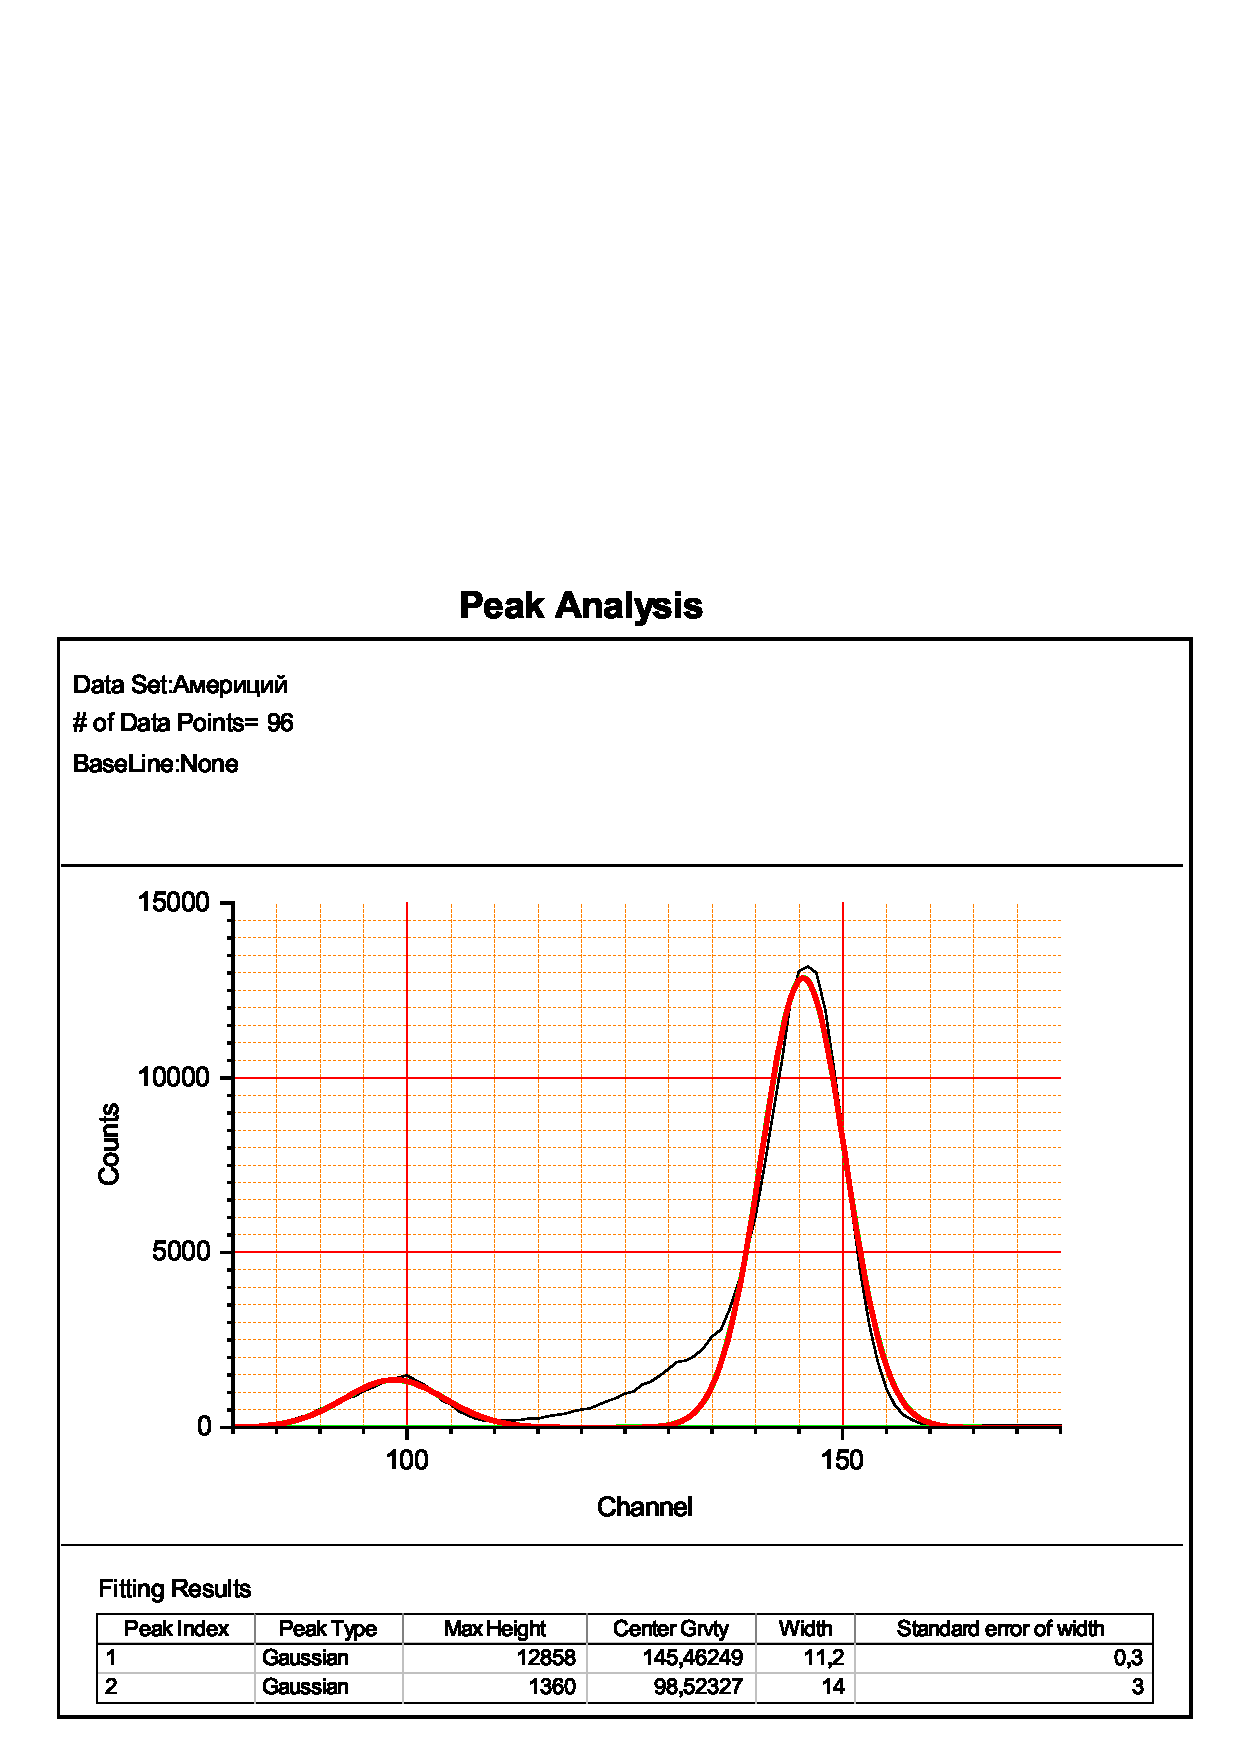
\includegraphics[width=0.80\textwidth]{5.png}\\
Иллюстрация, не является измерением.
\end{center}

В результате получилось

\[d_{\text{мех}}=(258-18)\pm1.1\,\text{мкм}=240\pm1.1\,\text{мкм}\]
\[d_{\text{опт}}=240\pm10\,\text{мкм}\]

\subsubsection*{12}

Для исследования дифракции Френеля на препятствии, поставим в место щели $S_2$ тонкую вертикальную нить и настроим микроскоп на ее резкое изображение

\begin{center}
\includegraphics[width=0.80\textwidth]{6.png}.\\
\end{center}

При удалении от нити всегда наблюдается четное число темных дифракционных полос.

\subsection{Дифракция Фраунгофера на щели}

\subsubsection*{1-3}
Для того, чтобы наблюдать дифракцию френеля, нужно поставить еще одну линзу $O_2$ после щели, чтобы в ее фокальной плоскости появилась картина из параллельных лучей. После этого достаточно настроить микроскоп на эту фокальную плоскость, сняв щель $S_2$ со скамьи и получив четкое изображение щели $S_1$ в окуляре.
\subsubsection*{4-7}
Пронаблюдаем дифракционную картину
\begin{center}
\includegraphics[width=0.80\textwidth]{7.png}.\\
\end{center}

\begin{center}
\begin{tabular}{|c|c|c|c|}\hline
$m$&$x_{min}\text{, \text{мм}}$&$x_{max}\text{, \text{мм}}$&$x\text{, \text{мм}}$\\\hline
$-5.0$&$0.26$&$0.38$&$0.320$\\\hline
$-4.0$&$0.54$&$0.64$&$0.590$\\\hline
$-3.0$&$0.80$&$0.90$&$0.850$\\\hline
$-2.0$&$1.08$&$1.18$&$1.130$\\\hline
$-1.0$&$1.36$&$1.42$&$1.390$\\\hline
$1.0$&$1.94$&$1.98$&$1.960$\\\hline
$2.0$&$2.16$&$2.28$&$2.220$\\\hline
$3.0$&$2.48$&$2.52$&$2.500$\\\hline
$4.0$&$2.72$&$2.86$&$2.790$\\\hline
$5.0$&$3.00$&$3.10$&$3.050$\\\hline
\end{tabular}\\~\\
$\Delta m=0\,\text{}, \Delta x_{min}=0.01\,\text{\text{мм}}, \Delta x_{max}=0.01\,\text{\text{мм}}, \Delta x=0.014\,\text{\text{мм}}$
\end{center}



\begin{center}
\includegraphics[width=0.80\textwidth]{8.png}.\\
\end{center}

Измерение проводились при ширине щели

\[D=(17.0\pm0.5)\times20\,\text{мкм}=340\pm10\,\text{мкм}.\]

И фокусном расстоянии линзы

\[f=160\,\text{мм}\]

Если $A = (274.0\pm0.9)\,\text{мкм}$ -- угол наклона графика, то
\[\lambda = D \frac{A}{f} = 582\pm19\,\text{нм}\]

\section*{Вывод}

Мы изучили два основных типа дифракции: Френеля и Фраунгофера при разных размерах щели и провели качественные наблюдения этих явлений, а также экспериментально проверили справедливость теоретических формул.  

\end{document}








\lipsum[1-4]
\begin{wrapfigure}{R}{5cm}
\centering
\includegraphics[width=0.20\textwidth]{rd.png}
\caption{1}
\end{wrapfigure}
\lipsum[1-6]


\begin{figure}[h]
\begin{center}$
\begin{array}{cccc}
\includegraphics[width=0.20\textwidth]{rd.png}&
\includegraphics[width=0.20\textwidth]{rd.png}&
\includegraphics[width=0.20\textwidth]{rd.png}&
\includegraphics[width=0.20\textwidth]{rd.png}\\
(1) & (2) & (3) & (4)
\end{array}$
\end{center}
\end{figure}
